\section{Background and Related Work} \label{section_bg_related}



\subsection{Passive Optical Network (PON)}


Compared to copper, optical fiber can provide higher bandwidth
over a longer distance. However, the deployment of optical fiber
in access networks is severely hindered by the cost issue.
%Unlike core networks that are shared by thousands/millions of users,
%the optical fibers and devices in a point-to-point optical access
%network cannot be shared among users and cost per capita is too high.
In fact, optical fiber was seriously considered for access
networks only after the emergence of PON technology.

\begin{figure}[!htbp]
\begin{center}
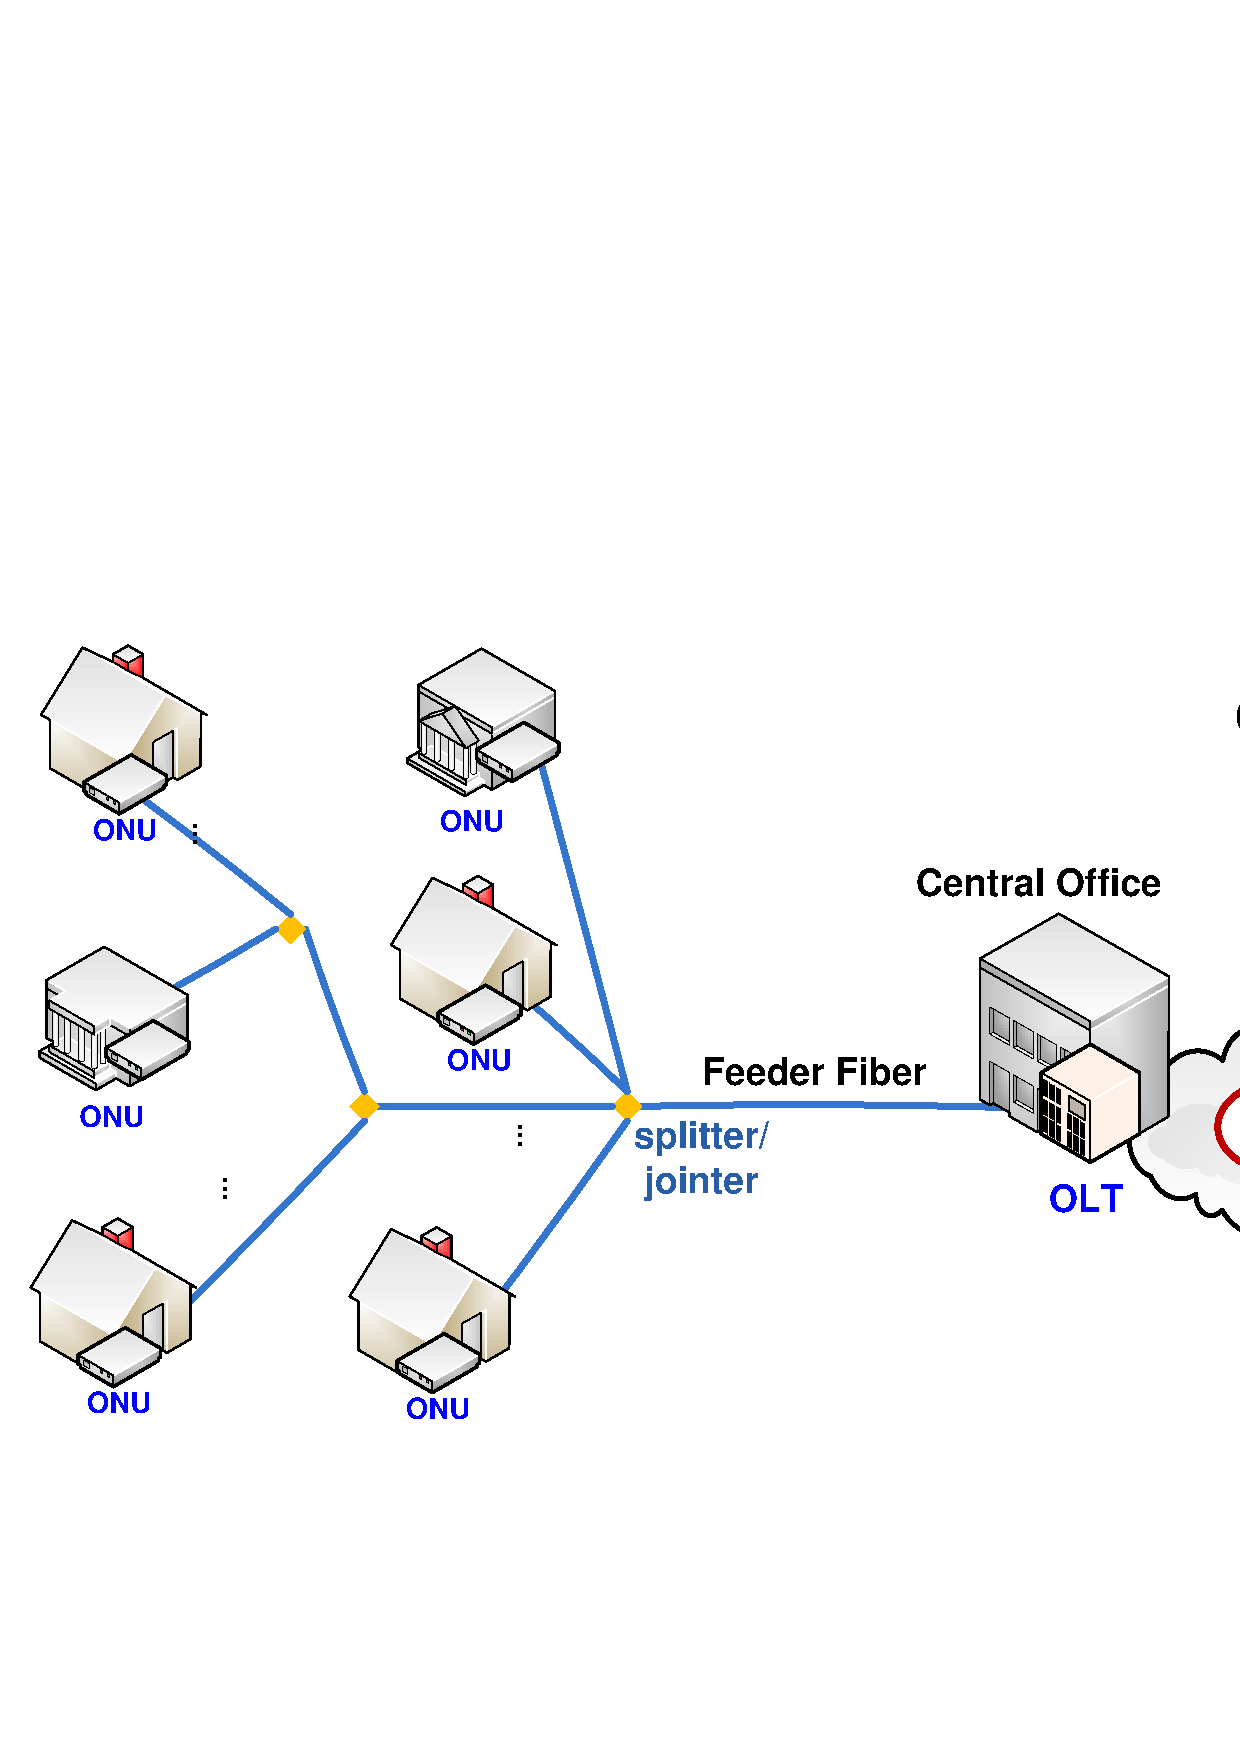
\includegraphics[ clip=true, trim=0mm 50mm 0mm 20mm, width=0.75\textwidth]{images/pon_bigger_font}
\end{center}
\vspace{-0.1in}
\caption{An Illustration of PON} \label{fig_pon}
\end{figure}

As shown in Figure \ref{fig_pon}, PON is a point-to-multipoint
fiber network and there are three kinds of equipment: the OLT
(Optical Line Terminal) in central office, ONUs (Optical Network
Unit) in/near customer premise, and passive optical
splitters/jointers in the middle. Through splitter/jointer, OLT
and the feeder fiber are shared by multiple users. Compared with
the point to point architecture, PON can significantly reduce the
amount of required optical fibers and the central office
equipments. Since the passive optical splitters/jointers do not
need power supply, the cost of deployment, maintenance and
operation can also be reduced. Thus, PON could reduce both capital
expenditure and operational expenditure significantly.

%It could be a feasible way (in economy) for some countries to provide high
%speed Internet access to end users.



In a classical TDMA (Time Division Multiple Access) based PON
network, downstream traffic is broadcast by the OLT to all ONUs
that share the same optical fiber and encryption is used to
prevent eavesdropping. Upstream traffic from ONUs is interleaved
by OLT for using the optical fiber in a TDMA-like manner. Since
ONUs normally have different distances to the OLT, the data bursts
from these ONUs must be scheduled carefully for providing a
collision-free and efficient upstream data communication. To
accommodate the dynamics in bandwidth demands from users and
exploit the gain of statistical multiplexing, dynamic bandwidth
assignment (DBA) is normally used for managing the upstream
bandwidth. More specifically, ONUs will report their buffer
occupancy to OLT, which will then allocate the upstream bandwidth
to ONUs based on their bandwidth demands and their Service Level
Agreement (SLA).


Some standards have been developed for PONs by both EFM of IEEE
(EPON) and FSAN of ITU-T (GPON). EPON is designed for carrying
Ethernet frames and GPON can carry various traffics through
encapsulation, such as Ethernet frames and ATM cells. Although
EPON and GPON have different frame structures, they share the same
network architecture and data communication follows the same
principles described above. %The physical reach of the existing
%PON-based networks is about 20 km, the supported data rate is
%around 1 Gb/s, and one fiber can be shared by 32 users.
One important difference between EPON and GPON is that GPON is
well standardized for QoS management. Hence, GPON can provide full
service with the same network and it is highly preferred by ISPs.
XG-PON is the new standard developed by FSAN  based on GPON. Its
details will be introduced in section \ref{section_xgpon}.

%GPON has dominated the FTTx market except in Japan.










\subsection{NS-3 Network Simulator}

NS-3 \cite{ns3} is a state of the art open-source network
simulator. Based on many lessons from the well-known NS-2
simulator \cite{ns2}, NS-3 is written from the scratch and it is a
completely new network simulator. NS-3 has many attractive
features, such as high emphasis on conformance to real networks,
good support for testbeds, a novel attribute system for
configuring simulation parameters, automatic memory management,
and a configurable tracing system \cite{henderson08ns3}. It has
also been reported that NS-3 performs much better than other
simulators in terms of simulation speed and memory overhead
\cite{weingartner09NS3Performance}. The first release of NS-3 was
made in June 2008 with support for a number of modules including
CSMA, Point-to-Point, WiFi (IEEE 802.11), TCP, UDP and IPv4.
Figure \ref{fig_ns3components} shows the organization of NS-3
modules.

\begin{figure}[!htbp]
\begin{center}
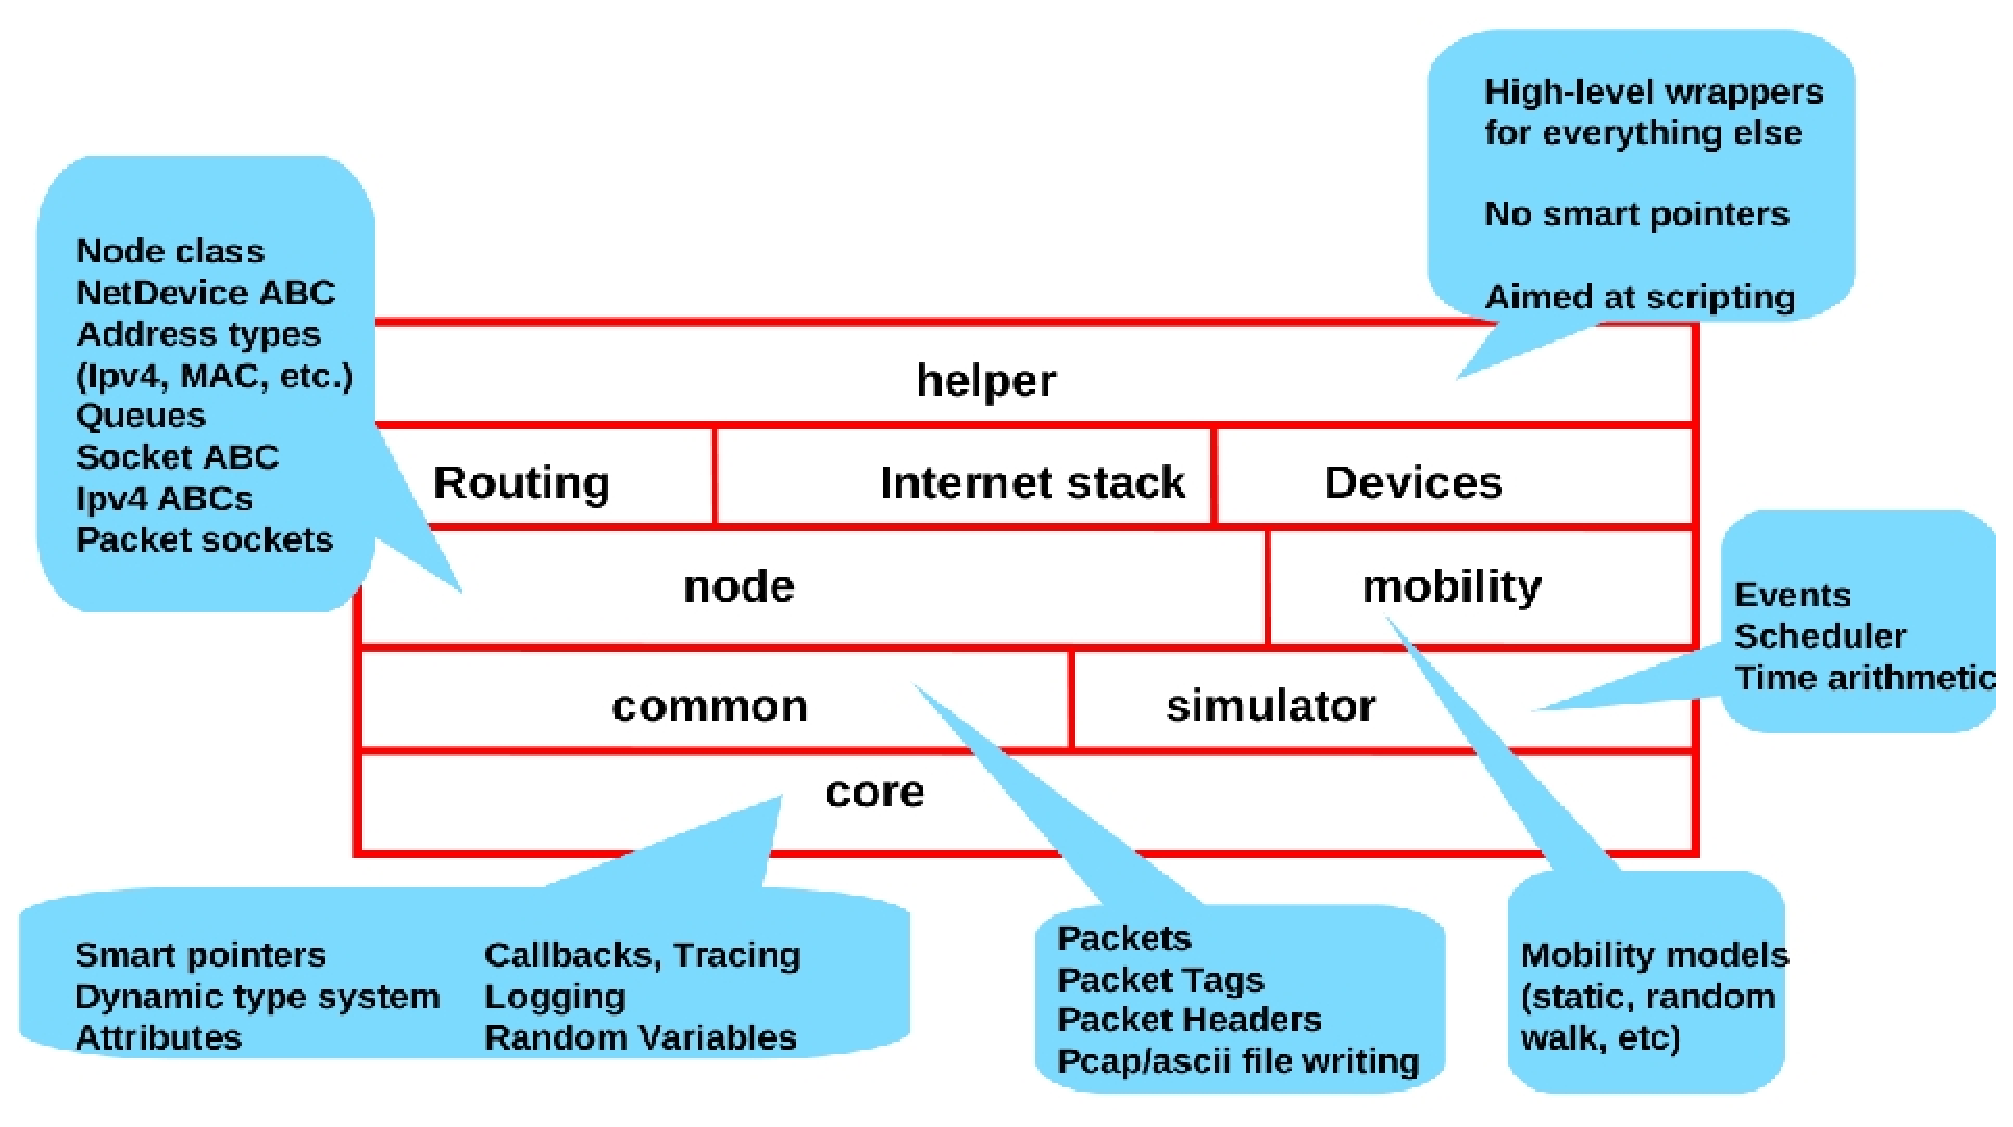
\includegraphics[width=0.75\textwidth]{images/ns3componnets}
\end{center}
\vspace{-0.1in}
\caption{The Organization of NS-3 Modules}
\label{fig_ns3components}
\end{figure}


In the last few years, many new modules have been developed and
added into NS-3, such as WiMAX module from Inria
\cite{farooq09wimax4ns3} and LTE module from CTTC
\cite{piro11lte4ns3}. Thus, through implementing one XG-PON module
in NS-3, we can get a very good research platform for studying the
issues arisen with the deployment of XG-PON.


\subsection{Related Work}

Although simulation has been used to study PON, the existing work
cannot be used directly or extended easily to study the
performance issues arising with the deployment of XG-PON.

In \cite{song09multithread4LRPON}, the authors developed their own
simulator to study dynamic bandwidth assignment (DBA) algorithms
when the physical reach is much longer than the current PON
networks. This simulator has limited functions and there is no
Internet protocol stack, which is needed to study many research
topics.

EPON and GPON had also been studied with OPNET \cite{opnet} and
several models have been implemented by different groups
\cite{chang08dba4GEPON}\cite{peng11epon4opnet}. However, these
EPON/GPON models are not available to the public. Furthermore,
OPNET simulates too many details (CPU of a router, etc.) and the
simulation speed is slow even when the simulated network bandwidth
is lower than 1 Gb/s. Since OPNET is not an open-source simulator,
we cannot change its core to simulate a 10 Gb/s XG-PON network
with a reasonable simulation speed.


In addition, one simple EPON module has been developed for OMNeT++
\cite{bodozoglou10epon4omnet} and the code is available to the
public. Since there are a lot of difference between EPON and
XG-PON, the code of this EPON module may not be very helpful to
implement one XG-PON module for OMNeT++. Considering the good
points of NS-3 discussed above, it should be better to develop one
XG-PON module from the scratch for the NS-3 network simulator.


Hence, an XG-PON module is designed and implemented in this report
for NS-3. With such an XG-PON module, we can simulate XG-PON and
study its own performance. With the more realistic Internet
protocol stack of NS-3, we can study the performance experienced
by users/applications in XG-PON networks. With the existing NS-3
modules for various wireless networks (WiFi, WiMAX, LTE, etc.), we
can also study the integration between XG-PON and wireless
networks, which is the trend of the future Internet access
networks. In summary, with this XG-PON module, NS-3 will become a
good platform for studying the next generation Internet access
networks composed by XG-PON and wireless networks.

Not only XG-PON, we can also extend this XG-PON module to study
Long-Reach PON (LR-PON), an evolution of XG-PON with a larger
number of users, symmetric data rate (10 Gb/s in both upstream and
downstream), and longer reach (100+ km)
\cite{payne02lrpon}\cite{shea07lrpon10G1000onu}. The aim of our
LR-PON research group is to initially build LR-PON from the XG-PON
standard, while identifying the required modifications and
improvements.
